\documentclass[tikz,border=10pt]{standalone}
\usepackage{tikz}
\usetikzlibrary{arrows.meta,positioning,calc,backgrounds,fit,shapes.geometric}
\usepackage[scaled=0.92]{helvet}
\renewcommand{\familydefault}{\sfdefault}
\usepackage{amsmath,amssymb}
\definecolor{ink}{HTML}{262624}
\definecolor{mute}{HTML}{8A8984}
\definecolor{line}{HTML}{BDBBB5}
\definecolor{acc}{HTML}{2A78D6}
\definecolor{accbg}{HTML}{F1F6FD}
\tikzset{
  >={Latex[length=2.2mm]},
  every node/.style={text=ink},
  b/.style={draw=line, fill=white, rounded corners=2pt, align=center, inner sep=6pt,
            minimum height=10mm, text width=#1, font=\small},
  b/.default=40mm,
  a/.style={b=#1, draw=acc, fill=accbg},
  a/.default=40mm,
  t/.style={font=\footnotesize, text=mute, align=center},
  e/.style={->, draw=mute, line width=0.6pt},
  ea/.style={->, draw=acc, line width=0.9pt},
  eh/.style={->, draw=acc, line width=0.9pt, dash pattern=on 3pt off 2pt},
}

\begin{document}
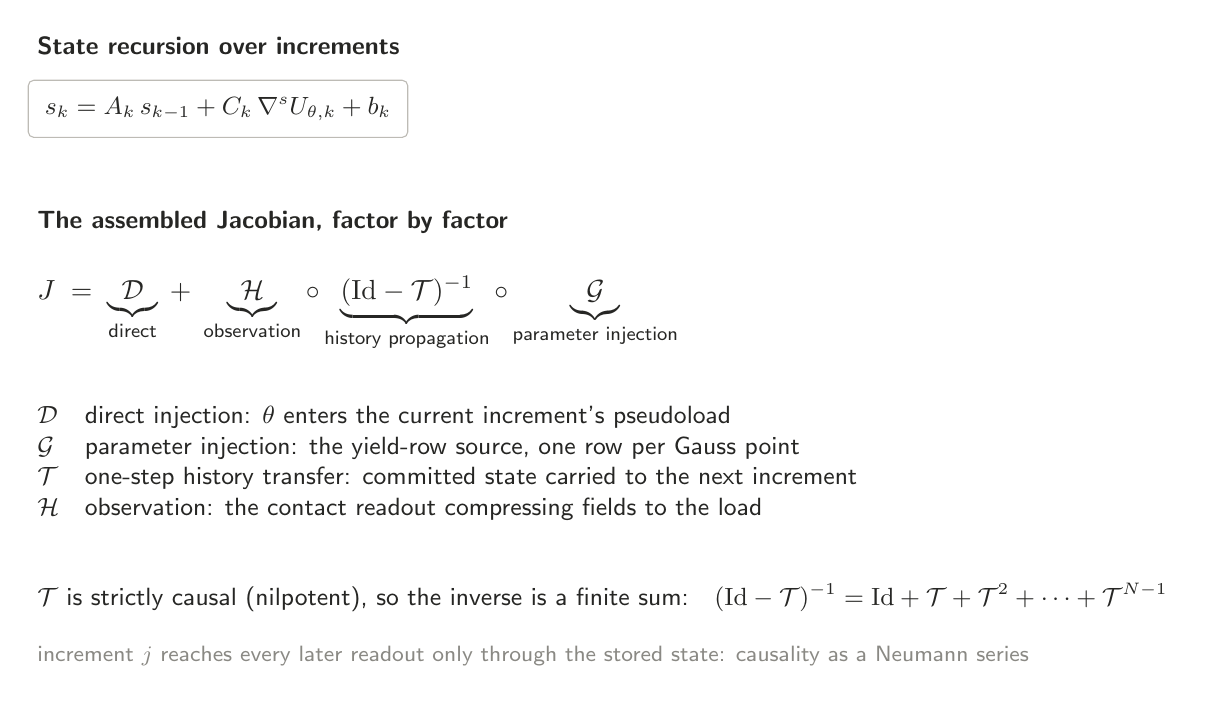
\begin{tikzpicture}
\node[anchor=north west, font=\small\bfseries] (h) at (0,0) {State recursion over increments};
\node[below=2mm of h.south west, anchor=north west, font=\small, draw=line, rounded corners=2pt, inner sep=6pt] (r) {$s_k = A_k\,s_{k-1} + C_k\,\nabla^s U_{\theta,k} + b_k$};
\node[below=8mm of r.south west, anchor=north west, font=\small\bfseries] (h2) {The assembled Jacobian, factor by factor};
\node[below=3mm of h2.south west, anchor=north west, font=\normalsize] (J) {%
$J \;=\; \underbrace{\mathcal D}_{\text{direct}} \;+\; \underbrace{\mathcal H}_{\text{observation}}\circ\underbrace{(\mathrm{Id}-\mathcal T)^{-1}}_{\text{history propagation}}\circ\underbrace{\mathcal G}_{\text{parameter injection}}$};
\node[below=4mm of J.south west, anchor=north west, font=\small, align=left] (L) {%
\begin{tabular}{@{}l@{\quad}l@{}}
$\mathcal D$ & direct injection: $\theta$ enters the current increment's pseudoload\\
$\mathcal G$ & parameter injection: the yield-row source, one row per Gauss point\\
$\mathcal T$ & one-step history transfer: committed state carried to the next increment\\
$\mathcal H$ & observation: the contact readout compressing fields to the load
\end{tabular}};
\node[below=5mm of L.south west, anchor=north west, font=\small, align=left] (N) {%
$\mathcal T$ is strictly causal (nilpotent), so the inverse is a finite sum:\quad
$(\mathrm{Id}-\mathcal T)^{-1} = \mathrm{Id} + \mathcal T + \mathcal T^2 + \cdots + \mathcal T^{N-1}$};
\node[below=2mm of N.south west, anchor=north west, t] {increment $j$ reaches every later readout only through the stored state: causality as a Neumann series};
\end{tikzpicture}
\end{document}
